\chapter{Predictive Coding}

\acf{PC} is the theory that the ``purpose'' of the perceptual system is not to encode the maximum amount of information about the current state of the world, but rather to provide a prediction of (the posterior distribution of) the future state of the world. 

Indeed, this provides a parsimonious explanation for much of the brain's function. If you consider a video of two people talking in a living room with an old TV displaying static - most of the Shannon information in the video will be in the TV's display. While the speck of static may be a result of a particle left by the big bang hitting the antenna, our brain doesn't devote the majority of its resources to keep track of the white noise patterns. i.e. the brain's sensory processing system isn't designed to maximize the mutual information between the sensory signals it receives. Instead, if you consider the temporal information, the brain tries to encode the predictive information within its sensory streams. \PC has been hailed by some as ``The unifying theory of the brain.''

\PC provided the inspiration and fundamental theory behind temporal difference learning, a class of model free reinforcement learning methods which learn by bootstrapping from the current prediction of the state of the world. Temporal Difference Learning produced TD-Gammon which was beating humans even before the more famous Deep Blue eventually beat Kasparaov. Temporal Difference Learning is also one of inspirations for many of the current state-of-the-art reinforcement learning applications such as AlphaGo by DeepMind and Five by OpenAI.

If we were prescribed to the theory of \PC we would expect that somewhere the brain has to encode 1) the prediction of what is to come, and 2) the error between the prediction and what actually came to pass. Indeed, some of the most famous work in neuroscience has demonstrated these values in predictions of reward in dopamine signalling in the VTA. However, the theory of \PC would expect that these values should exist throughout the perceptual system as well for all aspects of the state of the world. A good place to look for this would be where the brain processes complex time-varying signals, namely, in auditory processing regions.

\comment{Surprise}

``Indeed, a model-free approach seems out of the question in the context of video processing, as it would take unreasonably too many data samples and hence unreasonably too long to accumulate sufficient data and allow accurate model-free estimation of the underlying probability density function (PDF) of the data.''\cite{itti2005principled}

This is no longer true with modern machine learning techniques and methods for handling significantly more data than was possible in 2005. Therefore I have spent some effort building some models that predict future posterior probability density function of spectrograms.

\section{Models}

\subsection{Deep mixture of beta distributions}
My first attempt was to create a neural network that, given a window of spectrogram, predict the probability distribution of each frequency band in the next time bin of the spectrogram. The network was optimized by maximizing the log likelihood of the model. I modelled the probability distribution as a mixture of 3 beta distributions. The network was two fully connected layers with an output for a weight, $w$, and the two beta distribution parameters, $\alpha$ and $\beta$, for each of the three beta distributions, for each of the frequency bins. This network was very ill-behaved and I spent considerable time implementing as many numerical analysis tricks to control and regularize the networks exploding values. Most were relatively simple and included but was not limited to gradient clipping, different beta distribution approximations, the log-sum-exp trick and even an added cost function tied to the standard deviation of the beta distributions to try to prevent them from becoming delta functions.

One interesting method I used was adversarial training \cite{goodfellow2014explaining,lakshminarayanan2017simple}. Given an input $x$ with target $y$, and loss $l(\theta, x, y)$(e.g. $-\log p_\theta(y|x)$) \cite{goodfellow2014explaining} proposes the fast gradient sign method which generates an adversarial example as $x' = x + \epsilon \sign(\nabla_x l(\theta, x, y))$ and using $x'$ to augment the dataset by treating $(x', y)$ as an additional training example. Intuitively, this can be interpreted as a smoothing method by smoothing the likelihood around the target of an $\epsilon$-neighborhood around the training examples. This helped a small amount but my networks still eventually got corrupted by NaNs. In my case where I'm predicting the likelihood of a full spectrogram slice, its possible adversarial training on my labels, $y$ might have also helped the stability. In the end, however, I began to strip away as many of the complexities of the network as I could to create a minimal viable network.

\subsection{Deep Gaussian prediction}
This minimum network was to simply predict each frequency band as a univariate Gaussian with a mean and a standard deviation, and let the network try and deal with any covariances. This network trained easily enough, but didn't do nearly as good of a job at predicting as the deep mixture of beta distributions networks that were stopped before being corrupted by NaNs. However, even with this poor performance I did notice peaks in the likelihood that corresponded to motif boundaries.

\subsection{Contrastive Predictive Coding}
The last method I have explored is \CPC\cite{CPC}. \CPC is a method that takes high dimensional time varying data, and attempts to do representation learning on it to provide a representation that captures the predictive information of the signal. They do this by encoding the high dimensional signal in a low dimensional latent space, $Z$, using an encoding network, and then feeding the latent space into a recurrent neural network which outputs a context in another latent space, $C$. $c_t$ is then used to linearly classify if a sample is actually the next time sample, or drawn from a distribution (I have used other random samples from the spectrogram). The whole model is learned end-to-end, providing an encoding information to a $Z$ space that both contains information that is useful for predictions, as well as information that is predictable. The model also provides the $C$ which also contains extra context from the past.

Figure \ref{fig:encoder} shows an example 8 dimensional $Z$ latent space learned by \CPC. It encodes all the predictive and predictable information contained in each spectrogram time slice. Noticable changes in the spectrogram are reflected in some way in the encoded dimensions. It would be interesting to see if it allocated its weights in a similar distribution as would be predicted by the mel frequency scale.

\begin{figure}[tbp] 
  \centering
  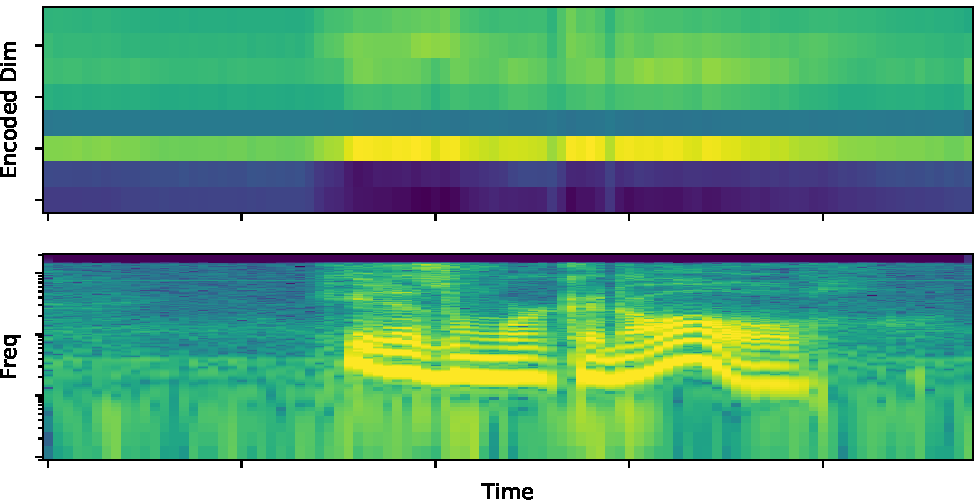
\includegraphics[width=\textwidth]{figures/encoder.pdf}
  \caption[8 dimensional $Z$ space learned by Contrastive Predictive Coding.]
{The representation learned by the encoder of \CPC. Top: The 8 dimensional latent space $Z$ created by pushing each spectogram time slice through the encoder network. Bottom: 2048 Frequency bin spectrogram representation (not log spaced) fed into the encoder and the \CPC network.
\index{encoder}}
  \label{fig:encoder}
\end{figure}

\subsection{Future Improvements}
\CPC seems to be working quite well to generate representations, even though it doesn't give us explicit predictions. It would be possible to extract predictions from the \CPC network by 1) sampling from the latent space, or 2) explicitly using the linear decision boundary created by the network. There are also several other changes that could be made to the architecture which may improve the performance. A Wavenet\cite{van2016wavenet} style time dilation network architecture might allow for the removal of the LSTM or recurrent neural network and might improve training time. Alternatively, a transformer network\cite{vaswani2017attention} might be more efficient recurrent neural network architecture that is still able to capture the necessary dynamics. Lastly, further skip-state predictions might improve the learned representations as hinted by \cite{gregor2018temporal}. There are many possible ways to incorporate skip state predictions into \CPC.

\section{Future Applications}

\subsection{Receptive Field Estimation}
These kinds of models have the potential to be used for much more than just posterior distribution prediction. As I alluded to in the introduction, an explicit model of the posterior distribution may allow for improved receptive field models and more accurate spike predictions. This would be done by splitting the stimuli explicitly into what was predicted, and how the actual stimuli differed from this prediction. Since the spiking could be dependent on the surprise at a variety of time lags, the dimensionality of this stimuli space quickly explodes as you consider farther back in time. To restrict the dimensions considered, a linear receptive field model should probably be used first to define the time lag limits and relevant frequency bands.

Alternatively, instead of using an explicit posterior prediction model, the learned \CPC encoded representation could be used to make spike predictions. This wouldn't require explicit arbitrary frequency limits which we have currently imposed by estimating the range of frequencies we believe the birds are sensitive to and by using a mel scale based on human cochlear organization. Furthermore, by varying the dimensionality of the \CPC encoded representation a balance between the encoded stimuli information and the limited experimental statistical power to combat the curse of dimensionality.

\subsection{Natural Unsupervised Segmentation of Vocal Objects}
Both word segmentation and motif segmentation has proven to be a non-trivial task and has limited efforts towards automatic vocal analysis. In both linguistics and birdsong research, hand segmentation remains the gold-standard technique for separating out vocal objects. For human speech, some supervised methods do a reasonable job, mainly due to large amounts of labeled data. For birdsong, this is not available.

Preliminary data seems to indicate the usefulness of the likelihood of each time sample as an unsupervised segmentation signal. Previous methods at song segmentation in our lab mainly consisted of using the sum of the spectral power for each time point. I suspect that an improved method could use the likelihood of each time sample or its derivative. This makes intuitive sense because one would expect that intra-object predictability to be higher than inter-object predictability.

\subsection{General Encoding of High-dimensional Time-Varying Data}
Lastly, these techniques might be useful to extract meaningful information out of general high-dimensional time-varying data, of which we have a lot in Neuroscience. I suspect that the success of techniques like Independent Components Analysis (ICA)\cite{ICA}, Delay Differential Analysis\cite{DDA}, and Taken's delay embeddings indicate the kinds of statistical structure that are utilized by \CPC are abundant and informative in Neuroscience data. I expect this to be useful for many types of recordings including but not limited to EEG, FMRI, Ecog, LFP, and even recordings of many single units, mainly as an unsupervised dimensionality reduction technique.